\documentclass[a4paper]{report}
\usepackage[utf8]{inputenc}
\usepackage[T1]{fontenc}
\usepackage[francais]{babel}
\usepackage{graphicx}
\usepackage{fullpage}
\usepackage{eso-pic}
 
\newcommand{\HRule}{\rule{\linewidth}{0.5mm}}
\newcommand{\blap}[1]{\vbox to 0pt{#1\vss}}
\newcommand\AtUpperLeftCorner[3]{%
  \put(\LenToUnit{#1},\LenToUnit{\dimexpr\paperheight-#2}){\blap{#3}}%
}
\newcommand\AtUpperRightCorner[3]{%
  \put(\LenToUnit{\dimexpr\paperwidth-#1},\LenToUnit{\dimexpr\paperheight-#2}){\blap{\llap{#3}}}%
}
 
\title{\LARGE{Stage chez Google France}}
\author{\textsc{Smith} John\\1A Spécialité Informatique\\Année universitaire 2013/2014}
\date{\today}
\makeatletter
 
\begin{document}
 
\begin{titlepage}
    \enlargethispage{2cm}
 
    \AddToShipoutPicture{
        \AtUpperLeftCorner{1.5cm}{1cm}{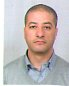
\includegraphics[width=4cm]{../img/redha.jpg}}
        \AtUpperRightCorner{1.5cm}{1cm}{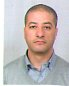
\includegraphics[width=6.5cm]{../img/redha.jpg}}
    }
 
    \begin{center}
        \vspace*{10cm}
 
        \textsc{\@title}
        \HRule
        \vspace*{0.5cm}
 
        \large{\@author} 
    \end{center}
 
    \vspace*{9.2cm}
 
    \begin{center}
        \makebox[\textwidth]{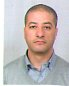
\includegraphics[width=\paperwidth]{../img/redha.jpg}}
    \end{center}
 
\end{titlepage}
\ClearShipoutPicture
 
\end{document}